\chapter{A Context-Free Top-Down Parser for Minimalist Grammars}
\label{cha:MG-TopDown}

Minimalist grammars are more powerful than CFGs, they generate mildly context-sensitive string languages, which are taken to be a good approximation of natural languages.
They are also very malleable and can be used as a formal basis for the overwhelming majority of analyses in the generative literature.
The question, however, is how MGs can be parsed.
In general, more powerful grammar formalisms require more sophisticated parsing strategies --- the higher expressivity comes at the cost of increased complexity.
As we will see today, however, MGs can actually be represented in terms of CFGs, which makes it a lot easier to design MG parsers based on the CFG parsers we already know.

\section{MG Derivations are Context-Free}
\label{sec:MG-TopDown_FeatureDerivationTrees}

The main difference between MG phrase structure trees and their corresponding derivation trees is that the latter only indicate when movement takes place, but no subtrees are actually being displaced.
Surprisingly, this minor difference has a big effect on the complexity of these two data structures.
Not all phrase structure trees can be generated by a context-free grammar --- if this were the case, MGs would not be any more powerful than CFGs.
MG derivation trees, however, are context-free.

Consider the following sentence from Bavarian German, which displays topicalization of the V-head.
%
\begin{exe}
    \ex {
        \gll  Gehauen hat der Hans die Maria (, nicht geküsst).\\
              beaten has the Hans the Maria (, not kissed).\\
        \glt `Hans beat Mary (he didn't kiss her).'
        }
\end{exe}
%
Since there are independent reasons to believe that the position before the finite verb can only be filled by phrases, the entire VP must have moved rather than the V-head itself.
But since the object DP \emph{die Maria} is part of the VP, it must have moved to a higher position outside the VP before the VP moved into the topic position.
Given standard Minimalist assumptions --- DP analysis of noun phrases, Larsonian shells, and the C-T-$v$-V clause spine --- the phrase structure tree thus should be similar to the one below (for the sake of simplicity we ignore head movement of the auxiliary verb from $v$ to T and C).
%
\begin{center}
    \begin{tikzpicture}
        \Tree
            [.CP
                [.\node(VP){VP$_v$};
                    [.V gehauen ]
                    \node(object_t){$t_o$};
                ]
                [.C$'$
                    [.C hat ]
                    [.TP
                        [.\node(subject){DP$_s$};
                            [.D der ]
                            [.N Hans ]
                        ]
                        [.T$'$
                            T
                            [.$v$P
                                [.\node(object){DP$_o$};
                                    [.D die ]
                                    [.N Maria ]
                                ]
                                [.$v$P
                                    \node(subject_t){$t_s$};
                                    [.$v'$
                                        $v$
                                        \node(VP_t){$t_v$};
                                    ]
                                ]
                            ]
                        ]
                    ]
                ]
            ]

        \clip (-9em,0) rectangle (17em,-25em);
        \draw[->,dashed] (VP_t.south west) .. controls +(225:8em) and +(190:15em) .. (VP.west);
        \draw[->,dashed] (subject_t.south) .. controls +(270:18em) and +(210:10em) .. (subject.west);
        \draw[->,dashed] (object_t.south) .. controls +(270:7em) and +(210:10em) .. (object.south west);
    \end{tikzpicture}
\end{center}
%
We can directly replicate this analysis with MGs.
%
\begin{center}
    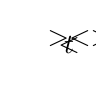
\begin{tikzpicture}
        \Tree
            [.$>$
                [.\node(VP){$<$};
                    \mlex{gehauen}{}
                    \node(object_t){$t$};
                ]
                [.$<$
                    \mlex{hat}{C}
                    [.$>$
                        [.\node(subject){$<$};
                            \mlex{der}{}
                            \mlex{Hans}{}
                        ]
                        [.$<$
                            \mlex{$\emptystring$}{}
                            [.$>$
                                [.\node(object){$<$};
                                    \mlex{die}{}
                                    \mlex{Maria}{}
                                ]
                                [.$>$
                                    \node(subject_t){$t$};
                                    [.$<$
                                        \mlex{$\emptystring$}{}
                                        \node(VP_t){$t$};
                                    ]
                                ]
                            ]
                        ]
                    ]
                ]
            ]
    \end{tikzpicture}

    \begin{tikzpicture}[
        level 1+/.style = { sibling distance = -9em },
        level 6/.style = { sibling distance = 2em },
        level 7/.style = { sibling distance = 0em },
        level 8/.style = { sibling distance = -3em },
        level 9/.style = { sibling distance = 0em }
        ]
        \Tree
            [.Move
                [.Merge
                    \mlex{hat}{\fsel{T}\ +top\ C}
                    [.Move
                        [.Merge
                            \mlex{$\emptystring$}{\fsel{\mathit{v}}\ +nom\ T}
                            [.Move
                                [.Merge
                                    [.\node(subject){Merge};
                                        \mlex{der}{\fsel{N}\ D\ -nom}
                                        \mlex{Hans}{N}
                                    ]
                                    [.Merge
                                        \mlex{$\emptystring$}{\fsel{V}\ \fsel{D}\ +acc\ \mathit{v}}
                                        [.\node(VP){Merge};
                                            \mlex{gehauen}{\fsel{D}\ V\ -top}
                                            [.\node(object){Merge};
                                                \mlex{die}{\fsel{N}\ D\ -acc}
                                                \mlex{Maria}{N}
                                            ]
                                        ]
                                    ]
                                ]
                            ]
                        ]
                    ]
                ]
            ]
    \end{tikzpicture}
\end{center}
%
At a quick glance it is actually hard to tell whether this derivation is well-formed.
That's because the derivation tree does not directly keep track of which features are still unchecked at each point of the derivation.
However, we can add this information by annotating every interior node with a tuple, each component of which is the list of unchecked features of some lexical item.
%
\begin{center}
    \begin{tikzpicture}[
        level 1+/.style = { sibling distance = -9em },
        level 6/.style = { sibling distance = 2em },
        level 7/.style = { sibling distance = 0em },
        level 8/.style = { sibling distance = -3em },
        level 9/.style = { sibling distance = 0em }
        ]
        \Tree
            [.\ftuple{C}
                [.\ftuple{+top\ C, -top}
                    \mlex{hat}{\fsel{T}\ +top\ C}
                    [.\ftuple{T, -top}
                        [.\ftuple{+nom\ T, -top, -nom}
                            \mlex{$\emptystring$}{\fsel{\mathit{v}}\ +nom\ T}
                            [.\ftuple{\mathit{v}, -top, -nom}
                                [.\ftuple{+acc\ \mathit{v}, -top, -acc, -nom}
                                    [.\ftuple{D\ -nom}
                                        \mlex{der}{\fsel{N}\ D\ -nom}
                                        \mlex{Hans}{N}
                                    ]
                                    [.\ftuple{\fsel{D}\ +acc\ \mathit{v}, -top, -acc}
                                        \mlex{$\emptystring$}{\fsel{V}\ \fsel{D}\ +acc\ \mathit{v}}
                                        [.\ftuple{V\ -top, -acc}
                                            \mlex{gehauen}{\fsel{D}\ V\ -top}
                                            [.\ftuple{D\ -acc}
                                                \mlex{die}{\fsel{N}\ D\ -acc}
                                                \mlex{Maria}{N}
                                            ]
                                        ]
                                    ]
                                ]
                            ]
                        ]
                    ]
                ]
            ]
    \end{tikzpicture}
\end{center}

Notice how the feature-annotated derivation tree can easily be described by a small number of rewrite rules:
%
\begin{center}
    \begin{tabular}{rcl}
        \ftuple{C}                                      & \rewrite & \ftuple{+top\ C, -top}\\
        \ftuple{+top\ C, -top}                          & \rewrite & \ftuple{\fsel{T}\ +top\ C} \ftuple{T, -top}\\
        \ftuple{T, -top}                                & \rewrite & \ftuple{+nom\ T, -top, -nom}\\
        \ftuple{+nom\ T, -top, -nom}                    & \rewrite & \ftuple{\fsel{\mathit{v}}\ +nom\ T} \ftuple{\mathit{v}, -top, -nom}\\
        \ftuple{\mathit{v}, -top, -nom}                 & \rewrite & \ftuple{+acc\ \mathit{v}, -top, -acc, -nom}\\
        \ftuple{+acc\ \mathit{v}, -top, -acc, -nom}     & \rewrite & \ftuple{D\ -nom} \ftuple{\fsel{D}\ +acc\ \mathit{v}, -top, -acc}\\
        \ftuple{D\ -nom}                                & \rewrite & \ftuple{\fsel{N}\ D\ -nom} \ftuple{N}\\
        \ftuple{\fsel{D}\ +acc\ \mathit{v}, -top, -acc} & \rewrite & \ftuple{\fsel{V}\ \fsel{D}\ +acc\ \mathit{v}} \ftuple{V\ -top, -acc}\\
        \ftuple{V\ -top, -acc}                          & \rewrite & \ftuple{\fsel{D}\ V\ -top} \ftuple{D\ -acc}\\
        \ftuple{D\ -acc}                                & \rewrite & \ftuple{\fsel{N}\ D\ -acc} \ftuple{N}\\[2em]
        %
        \ftuple{\fsel{T}\ +top\ C}                      & \rewrite & hat\\
        \ftuple{\fsel{\mathit{v}}\ +nom\ T}             & \rewrite & $\emptystring$\\
        \ftuple{\fsel{V}\ \fsel{D}\ +acc\ \mathit{v}}   & \rewrite & $\emptystring$\\
        \ftuple{\fsel{D}\ V\ -top}                      & \rewrite & gehauen\\
        \ftuple{\fsel{N}\ D\ -nom}                      & \rewrite & der\\
        \ftuple{\fsel{N}\ D\ -acc}                      & \rewrite & die\\
        \ftuple{N}                                      & \rewrite & Hans | Maria
    \end{tabular}
\end{center}
%
While these rewrite rules are incredibly difficult to make sense of for humans, they generate the desired derivation tree (with the minor difference that for the sake of readability every lexical item has been split into two nodes, with the phonetic exponent as the daughter of the feature component).
In fact, there is a fully automatic procedure for converting an MG $G$ with lexicon $\Lex$ into a CFG $C$ such that $C$ generates all well-formed derivation trees of $G$, and only those (this result hinges on the SMC; see \citealt{Kobele.etal07} and section 2.1.3 of \citealt{Graf13Thesis}).

Clearly every phrase structure tree is fully described by its derivation tree (or trees, if there are multiple ways of building and one and the same phrase structure tree), since the latter is a set of instructions for building the former.
This means that the structure of a sentence is completely specified by assigning it a derivation tree.
So even though an MG parser has to work for string languages that are not context-free, it still only has to assign each sentence a context-free structure -- the derivation trees.
As we will see next, this idea works fairly well, but there is one major complication: the string yield of a derivation tree does not correspond to the sentence being parsed because movement can change the order of words.

\section{Top-Down Parser with Feature Annotated Derivations}
\label{sec:MG-TopDown_Parser}

\subsection{MGs without Movement --- A Naive Top-Down Parser}
\label{sub:MG-TopDown_Naive}
For an MG without movement --- i.e.\ an MG where no lexical item has any licensee features --- designing a parser is straight-forward.
In this case, the order of the leaves in the derivation tree can be taken to mirror the order of the words in the input sentence.
So if MG $G$ is movement-free, we can translate it into a CFG that generates $G$'s derivation trees and use any one of our familiar parsers for this CFG\@.

But let's see if we can design a parser that reflects the MG feature calculus more directly.
If there are only Merge nodes in the derivation, every interior node has exactly two daughters.
In addition, all the features of the node must have been contributed by exactly one of its daughters, namely the one with the selector feature (take a minute to convince yourself that this is indeed the case!).
Since the selector may be linearized either to the left or to the right, we need two distinct inference rules.
%
\begin{prooftree}
    \AxiomC{\tuple{\alpha}}
    \LeftLabel{\textbf{Merge1}\qquad}
    \RightLabel{$F$ a feature name of $G$}
    \UnaryInfC{\tuple{\fsel{F}\ \alpha} \qquad \tuple{\mathrm{F}}}
\end{prooftree}
%
\begin{prooftree}
    \AxiomC{\tuple{\alpha}}
    \LeftLabel{\textbf{Merge2}\qquad}
    \RightLabel{$F$ a feature name of $G$}
    \UnaryInfC{\tuple{\mathrm{F}} \qquad \tuple{\fsel{F}\ \alpha}}
\end{prooftree}

There is one minor problem with those rules, though, and that's that the selector should always be to the left of its first argument, and always to the right of its other arguments.
Our rules do not capture this fact.
For example, if $\alpha$ is C then the parser could linearize the complementizer to the left or to the right of TP\@.
But an MG would only entertain the first option.
The simplest fix is to annotate each selector feature with information about how the argument is linearized, and that's the solution we will use for now.

\begin{prooftree}
    \AxiomC{\tuple{\alpha}}
    \LeftLabel{\textbf{Merge Right}\qquad}
    \RightLabel{F a feature name of $G$}
    \UnaryInfC{\tuple{\fsel{F}_r\ \alpha} \qquad \tuple{\mathrm{F}}}
\end{prooftree}
%
\begin{prooftree}
    \AxiomC{\tuple{\alpha}}
    \LeftLabel{\textbf{Merge Left}\qquad}
    \RightLabel{F a feature name of $G$}
    \UnaryInfC{\tuple{\mathrm{F}} \qquad \tuple{\fsel{F}_l\ \alpha}}
\end{prooftree}

The only thing remaining, then, is a rule for the removal of lexical items, similar to the scan rule.
%
\begin{prooftree}
    \AxiomC{\tuple{\alpha}}
    \LeftLabel{\textbf{LI}\qquad}
    \RightLabel{$\mlex{w}{\alpha} \in \Lex_G$}
    \UnaryInfC{}
\end{prooftree}

\subsection{Recursive Descent Parser for Movement-Free MGs}
\label{sub:MG-TopDown_Movement-Free}
The previous discussion is sufficient to outline the feature-based logic of an MG parser, but it does not serve as a parsing schema.
Just like in recursive descent parsing, our parsing items need to keep track of all the non-terminal symbols and put the in the right linear order.
This, however, is very simply to do.
%
For a recursive-descent MG parser, the only axiom is $[0,\psep \ftuple{C}]$, and the only goal is $[n,\psep]$.
%
\begin{prooftree}
    \AxiomC{$[i,\psep \tuple{\alpha} \beta, j]$}
    \LeftLabel{\textbf{Merge Left}\qquad}
    \RightLabel{F a feature name of $G$}
    \UnaryInfC{$[i,\psep \tuple{\mathrm{F}} \tuple{\fsel{F}_l\ \alpha} \beta, j]$}
\end{prooftree}
%
\begin{prooftree}
    \AxiomC{$[i,\psep \tuple{\alpha} \beta, j]$}
    \LeftLabel{\textbf{Merge Right}\qquad}
    \RightLabel{F a feature name of $G$}
    \UnaryInfC{$[i,\psep \tuple{\fsel{F}_r\ \alpha} \tuple{\mathrm{F}} \beta, j]$}
\end{prooftree}
%
\begin{prooftree}
    \AxiomC{$[i,\psep \tuple{\alpha} \beta, j]$}
    \LeftLabel{\textbf{LI (pronounced)}\qquad}
    \RightLabel{$\mlex{$w_i$}{\alpha} \in \Lex_G$, $w_i \neq \emptystring$}
    \UnaryInfC{$[i+1,\psep \beta, j]$}
\end{prooftree}
%
\begin{prooftree}
    \AxiomC{$[i,\psep \tuple{\alpha} \beta, j]$}
    \LeftLabel{\textbf{LI (empty)}\qquad}
    \RightLabel{$\mlex{$w_i$}{\alpha} \in \Lex_G$, $w_i = \emptystring$}
    \UnaryInfC{$[i,\psep \beta, j]$}
\end{prooftree}

\begin{examplebox}[MG Top-Down Parse of \emph{The man likes Mary}]
    Suppose the sentence \emph{The man likes Mary} has the structure below.
    %
    \begin{center}
        \begin{tikzpicture}
            \Tree
                [.CP
                    C
                    [.VP
                        [.DP
                            the
                            man
                        ]
                        [.V$'$
                            likes
                            [.DP
                                Mary
                            ]
                        ]
                    ]
                ]
        \end{tikzpicture}
    \end{center}
    %
    The feature-annotated Minimalist derivation tree for this sentence looks as follows.
    %
    \begin{center}
        \begin{tikzpicture}
            \Tree
                [.\ftuple{C}
                    \mlex{\emptystring}{\fsel{V}_r\ C}
                    [.\ftuple{V}
                        [.\ftuple{D}
                            \mlex{the}{\fsel{N}_r\ D}
                            \mlex{man}{N}
                        ]
                        [.\ftuple{\fsel{D}_l\ V}
                            \mlex{likes}{\fsel{D}_r\ \fsel{D}_l\ V}
                            \mlex{Mary}{D}
                        ]
                    ]
                ]
        \end{tikzpicture}
    \end{center}
    %
    The parse table directly reflects this structure.
    %
    \begin{center}
        \begin{tabular}{r|l}
            \textbf{parse item} & \textbf{inference rule}\\
                $\lbrack$0, \psep \ftuple{C}] & axiom\\
                $\lbrack$0, \psep \ftuple{\fsel{V}_r\ C} \ftuple{V}] & Merge Right\\
                $\lbrack$0, \psep \ftuple{V}] & LI (empty)\\
                $\lbrack$0, \psep \ftuple{D} \ftuple{\fsel{D}_l\ V}] & Merge Left\\
                $\lbrack$0, \psep \ftuple{\fsel{N}\ D} \ftuple{N} \ftuple{\fsel{D}_l\ V}] & Merge Right\\
                $\lbrack$1, \psep \ftuple{N} \ftuple{\fsel{D}_l\ V}] & LI (pronounced)\\
                $\lbrack$2, \psep \ftuple{\fsel{D}_l\ V}] & LI (pronounced)\\
                $\lbrack$2, \psep \ftuple{\fsel{D}_r \fsel{D}_l\ V} \ftuple{D}] & Merge Right\\
                $\lbrack$3, \psep \ftuple{D}] & LI (pronounced)\\
                $\lbrack$4, \psep ] & LI (pronounced)\\
        \end{tabular}
    \end{center}
    %
    We can annotate the final derivation tree as usual to indicate how it is built by the parser.
    %
    \begin{center}
        \begin{tikzpicture}
            \Tree
                [.\Lab{Merge}{1}{2}
                    \Lab{\mlex{\emptystring}{\fsel{V}_r\ C}}{2}{3}
                    [.\BLab{Merge}{2}{4}
                        [.\Lab{Merge}{4}{5}
                            \Lab{\mlex{the}{\fsel{N}_r\ D}}{5}{6}
                            \BLab{\mlex{man}{N}}{5}{7}
                        ]
                        [.\BLab{\ftuple{\fsel{D}_l\ V}}{4}{8}
                            \Lab{\mlex{likes}{\fsel{D}_r\ \fsel{D}_l\ V}}{8}{9}
                            \BLab{\mlex{Mary}{D}}{8}{10}
                        ]
                    ]
                ]
        \end{tikzpicture}
    \end{center}
\end{examplebox}

\subsection{Adding Movement}
\label{sub:MG-TopDown_Movement}
In principle, movement inference rules aren't all that different from Merge inference rules: we have a given expression of features, and infer which expressions this could have been produced from.
But there are three important differences:
%
\begin{itemize}
    \item Move is a unary rule, so we go from $\ftuple{\alpha}$ to $\ftuple{\beta}$, where $\beta$ differs minimally from $\alpha$,
    \item a tuple can now contain multiple feature strings, all but one of which are sequences of licensee features,
    \item we need a way to incorporate how Move changes the linear order of lexical items.
\end{itemize}
%
Let's deal with points 1 and 2 first.
In general, our feature tuples will now have the form $\ftuple{\alpha, \beta_1, \ldots, \beta_n}$, where each $\beta_i$ is a string of licensee features.
This means that we have to slightly change our Merge rules.
%
\begin{prooftree}
    \AxiomC{\tuple{\alpha, \beta_1, \ldots, \beta_n}}
    \LeftLabel{\textbf{Merge Right}\qquad}
    \RightLabel{F a feature name of $G$}
    \UnaryInfC{\tuple{\fsel{F}_r\ \alpha, \gamma_1, \ldots, \gamma_k} \qquad \tuple{\mathrm{F} \delta, \gamma_{k+1}, \ldots, \gamma_n}}
\end{prooftree}
%
\begin{prooftree}
    \AxiomC{\tuple{\alpha, \beta_1, \ldots, \beta_n}}
    \LeftLabel{\textbf{Merge Left}\qquad}
    \RightLabel{F a feature name of $G$}
    \UnaryInfC{\tuple{\mathrm{F} \delta, \gamma_1, \ldots, \gamma_k} \qquad \tuple{\fsel{F}_l\ \alpha, \gamma_{k+1}, \ldots, \gamma_n}}
\end{prooftree}
%
Notice that we now distribute the strings of licensee features over the two daughters of a Merge node in a non-deterministic fashion.
That is to say, we require in both rules that
%
\begin{itemize}
    \item for all $1 \leq i, j \leq n$, the first features of $\beta_i$ and $\beta_j$ are distinct,
    \item if $\delta = \emptystring$, then each $\beta_i$ is identical to exactly one $\gamma_j$, and \emph{vice versa},
    \item otherwise, there is some $\beta_i$ such that $\beta_i = \delta$ and the previous condition holds for all $\beta_j$ with $j \neq i$.
\end{itemize}

The logic of the movement rule is even simpler.
%
\begin{prooftree}
    \AxiomC{\tuple{\alpha, \beta_1, \ldots, \beta_i, \ldots, \beta_n}}
    \LeftLabel{\textbf{Move}\qquad}
    \RightLabel{$\mathrm{-f}$ a licensee feature of $G$}
    \UnaryInfC{\tuple{\mathrm{+f}\ \alpha, \beta_1, \ldots, \mathrm{-f}\ \beta_i, \ldots, \beta_n}}
\end{prooftree}
%
Notice that $\beta_i$ may be empty.
In that case, we are dealing with the final landing site of whichever lexical item hosts the $\mathrm{-f}$ feature.
Strictly speaking, then, the item in the antecedent line of the rule would have two adjacent commas with nothing inbetween the two since $\beta_i$ is empty.
Our rules never create an item of this form, so the Move rule couldn't apply in this case.
Hence we should actually distinguish two cases of movement.

\begin{prooftree}
    \AxiomC{\tuple{\alpha, \beta_1, \ldots, \beta_i, \ldots, \beta_n}}
    \LeftLabel{\textbf{Move (intermediate)}\qquad}
    \RightLabel{$\mathrm{-f}$ a licensee feature of $G$}
    \UnaryInfC{\tuple{\mathrm{+f}\ \alpha, \beta_1, \ldots, \mathrm{-f}\ \beta_i, \ldots, \beta_n}}
\end{prooftree}
%
\begin{prooftree}
    \AxiomC{\tuple{\alpha, \beta_1, \ldots, \beta_{i-1}, \beta_{i+1} \ldots, \beta_n}}
    \LeftLabel{\textbf{Move (final)}\qquad}
    \RightLabel{$\mathrm{-f}$ a licensee feature of $G$}
    \UnaryInfC{\tuple{\mathrm{+f}\ \alpha, \beta_1, \ldots, \beta_{i-1}, \mathrm{-f}, \beta_{i+1} \ldots, \beta_n}}
\end{prooftree}

These movement rules do not take care of the true challenge posed by movement however, and that's keeping track of the order of words in the sentence, which no longer corresponds to the order of words in the derivation tree.
Assume that we conjecture a Move node for topicalization.
Then we have to keep track of the fact that we expect to see an LI later on, which is handled by the presence of $\mathrm{-f}$ or $\mathrm{-f}\ \beta_i$ in the tuples.
But we also need to know that once we have found this item, the phrase it is a head of should match a sequence of words at the position where we initially conjectured topicalization movement.

\subsection{Keeping Track of Conjectured Movers}
\label{sub:MG-TopDown_MoveIndices}
In order to keep track of which positions in the string are associated with movers, we use place holders of the form $[f]$, where $f$ is a feature name.
These place holders are introduced by Move rules and allow us to reorder the tuples in a parse item where possible.
Given a substring $\phi$ of a parse item, $\phi_{/[f_1 \cdots f_n]}$ is the result of removing the placeholders $[f_1]$, \ldots, $[f_n]$ from $\phi$.

Once again the axiom is $[0,\psep \ftuple{C}]$ and the goal is $[n,\psep]$.
We need 4 Merge rule, 2 Move rules, and a few ancillary rules.
The Merge rules are parameterized according to linearization and whether the merged item is a mover.
%
\begin{prooftree}
    \AxiomC{$[i,
        \phi \psep
        \tuple{\alpha, \beta_1, \ldots, \beta_n}
        \psi
        ]$}
    \LeftLabel{\textbf{Merge Right}\qquad}
    \UnaryInfC{$[i,
        \phi
        \psep
        \tuple{\fsel{F}_r\ \alpha, \gamma_1, \ldots, \gamma_k}
        \tuple{\mathrm{F} \delta, \gamma_{k+1}, \ldots, \gamma_n}
        \psi
        ]$}
\end{prooftree}
%
\begin{prooftree}
    \AxiomC{$[i,
        \phi
        \psep
        \tuple{\alpha, \beta_1, \ldots, \beta_n}
        \psi
        ]$}
    \LeftLabel{\textbf{Merge Left}\qquad}
    \UnaryInfC{$[i,
        \phi
        \psep
        \tuple{\mathrm{F} \delta, \gamma_{k+1}, \ldots, \gamma_n}
        \tuple{\fsel{F}_l\ \alpha, \gamma_1, \ldots, \gamma_k}
        \psi
        ]$}
\end{prooftree}
%
\noindent
\textbf{Merge Mover Right}
\begin{prooftree}
    \AxiomC{$[i,
        \phi \psep
        \tuple{\alpha, \beta_1, \ldots, f_1 \cdots f_m, \beta_n}
        \psi
        ]$}
    \UnaryInfC{$[i,
        \phi_{/[f_1 \cdots f_{m-1}]}
        \psep
        \tuple{\fsel{F}_r\ \alpha, \gamma_1, \ldots, \gamma_{k-1}}
        [_{f_m} \tuple{\mathrm{F}\ f_1 \cdots f_m , \gamma_{k+1}, \ldots, \gamma_n}]
        \psi_{/[f_1 \cdots f_{m-1}]}
        ]$}
\end{prooftree}
%
\noindent
\textbf{Merge Mover Left}
\begin{prooftree}
    \AxiomC{$[i,
        \phi
        \psep
        \tuple{\alpha, \beta_1, \ldots, f_1 \cdots f_m , \ldots \beta_n}
        \psi
        ]$}
    \UnaryInfC{$[i,
        \phi_{/[f_1 \cdots f_{m-1}]}
        \psep
        [_{f_m} \tuple{\mathrm{F} f_1 \cdots f_n, \gamma_{k+1}, \ldots, \gamma_n}]
        \tuple{\fsel{F}_l\ \alpha, \gamma_1, \ldots, \gamma_{k-1}}
        \psi_{/[f_1 \cdots f_{m-1}]}
        ]$}
\end{prooftree}
%
The $f$-subscripted brackets around a tuple mark it as an $f$-mover, which is necessary to identify it with the right placeholder in $\phi$ or $\psi$.
Notice also that we eliminate all placeholders for intermediate movement as soon as the mover is merged.
Since the mover will never occur at an intermediate landing site --- after all, it has to move to its final target position --- those placeholders are string vacuous.
However, we have to introduce them first to make sure that the feature checking requirements are satisfied: every non-final licensee feature needs a corresponding move node, which corresponds to a placeholder in the parse item.

\begin{prooftree}
    \AxiomC{$[i,
        \phi
        \psep
        \tuple{\alpha, \beta_1, \ldots, \beta_i, \ldots, \beta_n}
        \psi
        ]$}
    \LeftLabel{\textbf{Move (intermediate)}\qquad}
    \UnaryInfC{$[i,
        \phi
        [\mathrm{f}]
        \psep
        \tuple{\mathrm{+f}\ \alpha, \beta_1, \ldots, \mathrm{-f}\ \beta_i, \ldots, \beta_n}
        \psi
        ]$}
\end{prooftree}
%
\begin{prooftree}
    \AxiomC{$[i,
        \phi
        \psep
        \tuple{\alpha, \beta_1, \ldots, \beta_{i-1}, \beta_{i+1} \ldots, \beta_n}
        \psi
        ]$}
    \LeftLabel{\textbf{Move (final)}\qquad}
    \UnaryInfC{$[i,
        \phi
        [\mathrm{f}]
        \psep
        \tuple{\mathrm{+f}\ \alpha, \beta_1, \ldots, \beta_{i-1}, \mathrm{-f}, \beta_{i+1} \ldots, \beta_n}
        \psi
        ]$}
\end{prooftree}
%
The Move rules are almost exactly the same, except that Move (intermediate) extends an existing $\beta_i$, whereas Move (final) adds a completely new one.

The actual reordering of tuples in a parse item is handled by the rule displace, which takes a mover and puts it in the position of the placeholder.
%
\begin{prooftree}
    \AxiomC{$[i,
        \phi [f] \phi'
        \psep
        [_f \alpha ]
        \psi
        ]$}
    \LeftLabel{\textbf{Displace Left}\qquad}
    \UnaryInfC{$[i,
        \phi \psep \alpha \phi'
        \psi
        ]$}
\end{prooftree}
%
\begin{prooftree}
    \AxiomC{$[i,
        \phi
        \psep
        [_f \alpha ]
        \psi
        [f]
        \psi'
        ]$}
    \LeftLabel{\textbf{Displace Right}\qquad}
    \UnaryInfC{$[i,
        \phi \psep \psi \alpha 
        \psi'
        ]$}
\end{prooftree}

The LI rule replaces a feature tuple by an LI with that feature specification, and the scan rule eliminates LIs from the parse items.
Scanning an LI is allowed only if it is at the very left edge of the parse item.
%
\begin{prooftree}
    \AxiomC{$[i,\phi \psep \tuple{\alpha} \psi]$}
    \LeftLabel{\textbf{LI}\qquad}
    \RightLabel{$\mlex{$a$}{\alpha} \in \Lex_G$}
    \UnaryInfC{$[i,\phi \psep a \psi]$}
\end{prooftree}
%
\begin{prooftree}
    \AxiomC{$[i,\psep a \beta]$}
    \LeftLabel{\textbf{Scan}\qquad}
    \RightLabel{$k = i$ if $a = \emptystring$ and $i+1$ otherwise}
    \UnaryInfC{$[k,\psep \beta]$}
\end{prooftree}

The shift rule moves $\psep$ to the right if no other rule can be applied.
%
\begin{prooftree}
    \AxiomC{$[i,
        \phi
        \psep x \psi
        ]$}
    \LeftLabel{\textbf{Shift}\qquad}
    \RightLabel{$\phi$ not the empty string, $x$ a placeholder or an LI}
    \UnaryInfC{$[i,
        \phi x
        \psep \psi
        ]$}
\end{prooftree}

\begin{examplebox}[MG Top-Down Parse of \emph{Gehauen hat die Maria der Hans}]
    Let's look at a slightly more complicated version of our very first example sentence.
    %
    \begin{exe}
        \ex
            {\gll Gehauen hat die Maria der Hans.\\
                  beaten has the Maria the Hans\\
            }
    \end{exe}
    %
    Here the object \emph{die Maria} not only moves out of the VP, but it also scrambles across the subject \emph{der Hans} afterwards.
    A simplified derivation tree is given below.
    %
    \begin{center}
        \begin{tikzpicture}
            \begin{scope}
                \tikzset{    
                    level 1+/.style = { sibling distance = -9em },
                    level 5+/.style = { sibling distance = 2em },
                }
                \Tree
                    [.\ftuple{C}
                        [.\ftuple{+top\ C, -top}
                            \mlex{hat}{\fsel{T}\ +top\ C}
                            [.\ftuple{T, -top}
                                [.\ftuple{+f\ T, -top, -f}
                                    [.\ftuple{+nom\ +f\ T, -top, -f, -nom}
                                        \mlex{$\emptystring$}{\fsel{\mathit{v}}\ +nom\ +f\ T}
                                        [.\ftuple{\mathit{v}, -top, -f, -nom}
                                            [.\ftuple{+acc\ \mathit{v}, -top, -acc\ -f, -nom}
                                                [.\ftuple{D\ -nom}
                                                    \mlex{der}{\fsel{N}\ D\ -nom}
                                                    \mlex{Hans}{N}
                                                ]
                                                \node(bottom){\phantom{bottom}};
                                            ]
                                        ]
                                    ]
                                ]
                            ]
                        ]
                    ]
            \end{scope}

            \begin{scope}[yshift=-27em]
                \Tree
                    [.\node(top){\ftuple{\fsel{D}\ +acc\ \mathit{v}, -top, -acc\ -f}};
                        \mlex{$\emptystring$}{\fsel{V}\ \fsel{D}\ +acc\ \mathit{v}}
                        [.\ftuple{V\ -top, -acc\ -f}
                            \mlex{gehauen}{\fsel{D}\ V\ -top}
                            [.\ftuple{D\ -acc\ -f}
                                \mlex{die}{\fsel{N}\ D\ -acc\ -f}
                                \mlex{Maria}{N}
                            ]
                        ]
                    ]
            \end{scope}

            \draw (top.north) .. controls +(45:2em) and +(270:8em) .. (bottom.north);
        \end{tikzpicture}
    \end{center}
    
    The parser infers the derivation with the following steps.
    %
    \begin{center}
        \small
        \begin{longtable}{r|l}
            \textbf{parse item} & \textbf{inference rule}\\
                $\lbrack$0, \psep \ftuple{C}] & axiom\\
                $\lbrack$0, [top] \psep \ftuple{+top\ C, -top}] & Move (final)\\
                $\lbrack$0, [top] \psep \ftuple{\fsel{T}\ +top\ C} \ftuple{T, -top}]  & Merge Right\\
                $\lbrack$0, [top] hat \psep \ftuple{T, -top}]  & LI \& Shift\\[.5em]
                %
                $\lbrack$0, [top] hat [f] &\\
                \psep \ftuple{+f\ T, -top, -f}]  & Move (final)\\[.5em]
                %
                $\lbrack$0, [top] hat [f] [nom] &\\
                \psep \ftuple{+nom\ +f\ T, -top, -f, -nom}] & Move (final)\\[.5em]
                %
                $\lbrack$0, [top] hat [f] [nom] &\\
                \psep \ftuple{\fsel{\mathit{v}}\ +nom\ +f\ T} \ftuple{\mathit{v}, -top, -f, -nom}] & Merge Right\\[.5em]
                %
                $\lbrack$0, [top] hat [f] [nom] \emptystring &\\
                \psep \ftuple{\mathit{v}, -top, -f, -nom}] & LI \& Shift\\[.5em]
                %
                $\lbrack$0, [top] hat [f] [nom] \emptystring\ [acc] \\
                \psep \ftuple{+acc\ \mathit{v}, -top, -acc\ -f, -nom}] & Move (intermediate)\\[.5em]
                %
                $\lbrack$0, [top] hat [f] [nom] \emptystring\ [acc] \\
                \psep [\tsb{nom} \ftuple{D\ -nom}] \ftuple{\fsel{D}\ +acc\ \mathit{v}, -top, -acc\ -f}] & Merge Mover Left\\[.5em]
                %
                $\lbrack$0, [top] hat [f] \psep \ftuple{D\ -nom} \emptystring\ [acc]\\
                \ftuple{\fsel{D}\ +acc\ \mathit{v}, -top, -acc\ -f}] & Displace Left\\[.5em]
                %
                $\lbrack$0, [top] hat [f] \psep \ftuple{\fsel{N}\ D\ -nom} \ftuple{N} \emptystring\ [acc]\\ 
                 \ftuple{\fsel{D}\ +acc\ \mathit{v}, -top, -acc\ -f}] & Merge Right\\[.5em]
                %
                $\lbrack$0, [top] hat [f] der \psep \ftuple{N} [f] [nom] \emptystring\ [acc]\\
                \ftuple{\fsel{D}\ +acc\ \mathit{v}, -top, -acc\ -f}] & LI \& Shift\\[.5em]
                %
                $\lbrack$0, [top] hat [f] der Hans \psep \emptystring\ [acc]\\
                \ftuple{\fsel{D}\ +acc\ \mathit{v}, -top, -acc\ -f}] & LI \& Shift\\[.5em]
                %
                $\lbrack$0, [top] hat [f] der Hans \emptystring\ [acc]\\
                \psep \ftuple{\fsel{D}\ +acc\ \mathit{v}, -top, -acc\ -f}] & Shift*2\\[.5em]
                %
                $\lbrack$0, [top] hat [f] der Hans \emptystring\ [acc]\\
                \psep \ftuple{\fsel{V}\ \fsel{D}\ +acc\ \mathit{v}} [\tsb{top} \ftuple{V\ -top, -acc\ -f}]] & Merge Mover Right\\[.5em]
                %
                $\lbrack$0, [top] hat [f] der Hans \emptystring\ [acc] \emptystring\\
                \psep [\tsb{top} \ftuple{V\ -top, -acc\ -f}]] & LI \& Shift\\[.5em]
                %
                $\lbrack$0, \psep \ftuple{V\ -top, -acc\ -f} hat [f] der Hans \emptystring\ [acc] \emptystring] & Displace Left\\[.5em]
                %
                $\lbrack$0, \psep \ftuple{\fsel{D}\ V\ -top} [\tsb{f} \ftuple{D\ -acc\ -f}]\\
                hat [f] der Hans \emptystring\ \emptystring] & Merge Mover Right\\[.5em]
                %
                $\lbrack$0, \psep gehauen [\tsb{f} \ftuple{D\ -acc\ -f}]\\
                hat [f] der Hans \emptystring\ \emptystring] & LI\\[.5em]
                %
                $\lbrack$1, \psep [\tsb{f} \ftuple{D\ -acc\ -f}]\\
                hat [f] der Hans \emptystring\ \emptystring] & Scan\\[.5em]
                %
                $\lbrack$1, \psep 
                hat \ftuple{D\ -acc\ -f} der Hans \emptystring\ \emptystring] & Displace Right\\[.5em]
                %
                $\lbrack$2, \psep 
                \ftuple{D\ -acc\ -f} der Hans \emptystring\ \emptystring] & Scan\\[.5em]
                %
                $\lbrack$2, \psep 
                \ftuple{\fsel{N}\ D\ -acc\ -f} \ftuple{N} der Hans \emptystring\ \emptystring] & Merge Right\\[.5em]
                %
                $\lbrack$2, \psep 
                die \ftuple{N} der Hans \emptystring\ \emptystring] & LI\\[.5em]
                %
                $\lbrack$3, \psep 
                \ftuple{N} der Hans \emptystring\ \emptystring] & Scan\\[.5em]
                %
                $\lbrack$3, \psep 
                Maria der Hans \emptystring\ \emptystring] & LI\\[.5em]
                %
                $\lbrack$4, \psep 
                der Hans \emptystring\ \emptystring] & Scan\\
                %
                $\lbrack$5, \psep 
                Hans \emptystring\ \emptystring] & Scan\\
                %
                $\lbrack$6, \psep 
                \emptystring\ \emptystring] & Scan\\
                %
                $\lbrack$6, \psep 
                \emptystring] & Scan\\
                %
                $\lbrack$6, \psep 
                ] & Scan\\
        \end{longtable}
    \end{center}

    We can represent this parse more succinctly by annotating the derivation tree with indices in the usual fashion.
    %
    \begin{center}
        \begin{tikzpicture}
            \begin{scope}
                \tikzset{    
                    level 1+/.style = { sibling distance = -9em },
                    level 6+/.style = { sibling distance = 0em },
                }
                \Tree
                    [.\Lab{Move}{1}{2}
                        [.\Lab{Merge}{2}{3}
                            \BLab{\mlex{hat}{\fsel{T}\ +top\ C}}{3}{13}
                            [.\Lab{Move}{3}{4}
                                [.\Lab{Move}{4}{5}
                                    [.\Lab{Merge}{5}{6}
                                        \BLab{\mlex{\emptystring}{\fsel{\mathit{v}}\ +nom\ +f\ T}}{6}{19}
                                        [.\Lab{Move}{6}{7}
                                            [.\Lab{Merge}{7}{8}
                                                [.\Lab{Merge}{8}{9}
                                                    \BLab{\mlex{der}{\fsel{N}\ D\ -nom}}{9}{17}
                                                    \BLab{\mlex{Hans}{N}}{9}{18}
                                                ]
                                                \node(bottom){\phantom{bottom}};
                                            ]
                                        ]
                                    ]
                                ]
                            ]
                        ]
                    ]
            \end{scope}

            \begin{scope}[yshift=-27em]
                \tikzset{
                    level 1+/.style = { sibling distance = -5em },
                    level 3/.style = { sibling distance = 0em}
                }
                \Tree
                    [.\node(top){\BLab{Merge}{8}{10}};
                        \BLab{\mlex{$\emptystring$}{\fsel{V}\ \fsel{D}\ +acc\ \mathit{v}}}{10}{20}
                        [.\Lab{Merge}{10}{11}
                            \Lab{\mlex{gehauen}{\fsel{D}\ V\ -top}}{11}{12}
                            [.\BLab{Merge}{11}{14}
                                \Lab{\mlex{die}{\fsel{N}\ D\ -acc\ -f}}{14}{15}
                                \BLab{\mlex{Maria}{N}}{14}{16}
                            ]
                        ]
                    ]
            \end{scope}

            \draw (top.north) .. controls +(45:2em) and +(270:12em) .. (bottom.north);
        \end{tikzpicture}
    \end{center}
\end{examplebox}

\subsection{Two Issues}
\label{sub:MG-TopDown_Issues}
The parser as defined in the previous section has two issues.
First, the Merge and Move rules are only limited by the requirement that the features $\mathrm{F}$ or $\mathrm{f}$ must be valid features of the grammar.
This, however, can still lead to conjecturing tuples that could never be derived from the LIs of the grammar.
These parses will eventually fail, of course, but for efficiency reasons it would be nice if the parser would not conjecture items that can never occur in a well-formed derivation.

If we translate the MG into a CFG, the set of valid tuples corresponds to the set non-terminals of the CFG.
So with a little bit of processing, the rules can be limited to only use non-terminals of this CFG\@.
It would be more appealing, however, if we could phrase our inference rules in a way so that they operate directly on the lexicon of our MG\@.
This is exactly what is done in \citet{Stabler12}.

\posscitet{Stabler12} parser also fixes another problem with the current model.
Right now, our parser does not sufficiently prioritize the search for movers.
Since scanning of an LI $l$ is delayed until all movers to the left of $l$ have been found, memory usage would be minimized by searching for those movers.
So once the parser stipulates the presence of a top-mover in the example above, it should first follow the branches that it believes will lead it to this mover.
Once this mover has been found, it can scan \emph{hat} and then continue it's search for an $\mathrm{f}$-mover, and then for a nom-mover.
Instead, our parser starts building the nom-mover before it has even found the top-mover; this increases the memory burden because there is no way the nom-mover could be fully scanned at this point.

\begin{examplebox}[A More Efficient Traversal of the Derivation Tree]
    Using the search strategy outlined in \citet{Stabler12}, the derivation tree from the previous example would be explored in the following order.

    \begin{center}
        \begin{tikzpicture}
            \begin{scope}
                \tikzset{    
                    level 1+/.style = { sibling distance = -9em },
                    level 6+/.style = { sibling distance = 0em },
                }
                \Tree
                    [.\Lab{Move}{1}{2}
                        [.\Lab{Merge}{2}{3}
                            \BLab{\mlex{hat}{\fsel{T}\ +top\ C}}{3}{12}
                            [.\Lab{Move}{3}{4}
                                [.\Lab{Move}{4}{5}
                                    [.\Lab{Merge}{5}{6}
                                        \BLab{\mlex{\emptystring}{\fsel{\mathit{v}}\ +nom\ +f\ T}}{6}{19}
                                        [.\Lab{Move}{6}{7}
                                            [.\Lab{Merge}{7}{8}
                                                [.\BLab{Merge}{8}{16}
                                                    \Lab{\mlex{der}{\fsel{N}\ D\ -nom}}{16}{17}
                                                    \BLab{\mlex{Hans}{N}}{16}{18}
                                                ]
                                                \node(bottom){\phantom{bottom}};
                                            ]
                                        ]
                                    ]
                                ]
                            ]
                        ]
                    ]
            \end{scope}

            \begin{scope}[yshift=-27em]
                \tikzset{
                    level 1+/.style = { sibling distance = -5em },
                    level 3/.style = { sibling distance = 0em}
                }
                \Tree
                    [.\node(top){\Lab{Merge}{8}{9}};
                        \BLab{\mlex{$\emptystring$}{\fsel{V}\ \fsel{D}\ +acc\ \mathit{v}}}{9}{20}
                        [.\Lab{Merge}{9}{10}
                            \Lab{\mlex{gehauen}{\fsel{D}\ V\ -top}}{10}{11}
                            [.\BLab{Merge}{10}{13}
                                \Lab{\mlex{die}{\fsel{N}\ D\ -acc\ -f}}{13}{14}
                                \BLab{\mlex{Maria}{N}}{13}{15}
                            ]
                        ]
                    ]
            \end{scope}

            \draw (top.north) .. controls +(45:2em) and +(270:12em) .. (bottom.north);
        \end{tikzpicture}
    \end{center}
    
    The Stabler parser has a lower payload because it does not fully expand the subject right away and instead moves on to the VP first.
    If the subject contained more than two LIs, the difference in payload would be even bigger.
    Maximum tenure stays the same because it is incurred at the T-head, which is introduced before the two parser diverge in their search path and cannot be scanned until the subject has been built and scanned.
    For this reason, the differences between the two parsers do not affect the node's tenure.
    We see a marked difference in summed tenure, however, because of the tenure contributed by \emph{der} and \emph{Hans}.
    %
    \begin{center}
        \begin{tabular}{rcc}
            \textbf{Metric} & \textbf{CF Parser} & \textbf{Stabler Parser}\\
            Payload & 8 & 7\\
            MaxTen & 13 & 13\\
            SumTen & 57 & 48
        \end{tabular}
    \end{center}
\end{examplebox}
%
\begin{exercise}
    Draw a movement-free Minimalist derivation tree for \emph{The anvil hit Daffy}.
    Assume a C-T-V spine where the subject is merged as the second argument of the T-head.
    The write down the parse table and annotate the derivation tree accordingly.
    Does the parser's behavior differ noticeably from what we observed for the recursive descent parser in Chapter~\ref{cha:TopDown}?
\end{exercise}
%
\begin{exercise}
    Following up on the previous exercise, assume that we actually have a C-T-$v$-V spine where the subject starts in Spec,$v$P and then moves to Spec,TP\@.
    Once again you have to write down the parse table and annotate the derivation tree.
    What differences do you observe?
\end{exercise}

\begin{exercise}
    Draw Minimalist derivation trees for our left-embedding and right-embedding analyses of \emph{John's father's car's exhaust pipe} disappeared.
    Assume a C-T-$v$-V spine where the subject moves from Spec,$v$P to Spec,TP\@.
    Then write down the parse table for each structure. 
    Annotate the derivation trees according to how our parser would build them.
    Is the behavior of our parser similar to that of the recursive descent parser?
\end{exercise}

\bibliographystyle{linquiry3}
\bibliography{universal,graf}
